\chapter{Solu\c tia propus\u a \c si arhitectura sistemului}

Acest capitol descrie arhitectura general\u a a aplica\c tiei Gym-Connect,
modelul de date, API-ul REST implementat \c si mecanismele de securitate
utilizate. Deciziile de proiectare sunt argumentate \^ in raport cu
cerin\c tele func\c tionale \c si nefunc\c tionale ale sistemului.
Diagramele prezentate \^ in acest capitol (arhitectur\u a, model de date,
secven\c t\u a \c si cazuri de utilizare) au fost realizate cu ajutorul
instrumentului \textbf{PlantUML} \cite{plantuml2024}, care permite
generarea diagramelor UML pornind de la o descriere textual\u a.

\section{Arhitectura general\u a}

Gym-Connect adopt\u a o arhitectur\u a clasic\u a de tip
\textbf{client-server}, \^ in care cele dou\u a componente principale
-- interfa\c ta utilizator (frontend) \c si serverul API (backend) --
ruleaz\u a independent \c si comunic\u a prin cereri HTTP.

Sistemul este compus din trei niveluri distincte, ilustrate \^ in
figura \ref{fig:arhitectura}:

\begin{figure}[htbp]
  \centering
  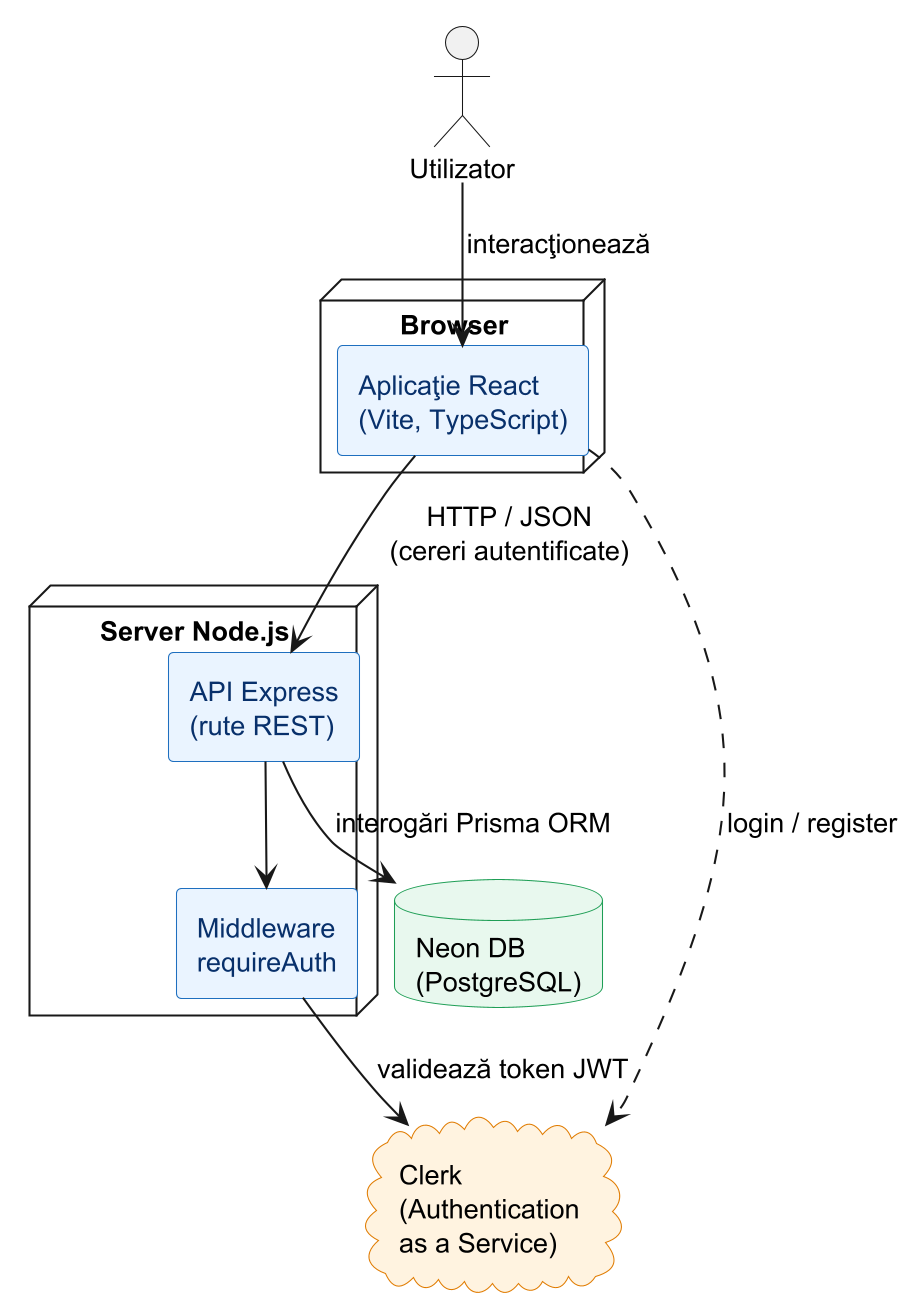
\includegraphics[width=0.72\textwidth]{arhitectura.png}
  \caption{Arhitectura general\u a a aplica\c tiei Gym-Connect}
  \label{fig:arhitectura}
\end{figure}

\begin{enumerate}
  \item \textbf{Nivelul de prezentare (Frontend)} -- aplica\c tia React
        care ruleaz\u a \^ in browserul utilizatorului. Aceasta
        gestioneaz\u a interfa\c ta utilizator, starea local\u a
        a aplica\c tiei \c si comunic\u a cu serverul prin cereri
        HTTP autentificate.

  \item \textbf{Nivelul de logic\u a de business (Backend)} -- serverul
        Express.js care ruleaz\u a pe Node.js. Acesta prime\c ste
        cererile de la client, le valideaz\u a, aplic\u a logica
        de business \c si interac\c tioneaz\u a cu baza de date
        prin Prisma ORM.

  \item \textbf{Nivelul de date (Baza de date)} -- instan\c ta
        PostgreSQL g\u azduit\u a pe platforma Neon DB. Stocheaz\u a
        toate datele aplica\c tiei: rutine de antrenament,
        sesiuni \c si seturi individuale.
\end{enumerate}

Fluxul standard al unei cereri este urm\u atorul: browserul
utilizatorului trimite o cerere HTTP c\u atre serverul Express,
\^ inso\c tit\u a de un token de autentificare Clerk. Serverul
valideaz\u a tokenul, proceseaz\u a cererea, interogheaz\u a
baza de date prin Prisma \c si returneaz\u a r\u aspunsul \^ in
format JSON c\u atre client.

\^ In modul de dezvoltare, Vite ofer\u a un \textbf{proxy} c\u atre
serverul backend, astfel \^ inc\^ at cererile de pe
\texttt{localhost:5173/api/*} sunt redirijate automat c\u atre
\texttt{localhost:3001/api/*}, evit\^ and problemele de CORS \^ in
timpul dezvolt\u arii.

\section{Modelul de date}

Schema bazei de date este definit\u a declarativ \^ in fi\c sierul
\texttt{prisma/schema.prisma} \c si este compus\u a din trei modele
principale, interconectate prin rela\c tii de tip
\textit{one-to-many}.

\subsection{Modelul SplitTemplate}

Modelul \texttt{SplitTemplate} reprezint\u a un \textbf{\c sablon de
rutin\u a de antrenament} -- un plan predefinit care descrie ce
exerci\c tii, c\^ ate seturi \c si ce interval de repeti\c tii
trebuie efectuate. Un utilizator poate crea oric\^ ate rutine,
iar fiecare rutin\u a apar\c tine exclusiv utilizatorului care
a creat-o.

\begin{table}[htbp]
\centering
\caption{C\^ ampurile modelului \texttt{SplitTemplate}}
\label{tab:split}
\begin{tabular}{|l|l|l|}
\hline
\textbf{C\^ amp} & \textbf{Tip} & \textbf{Descriere} \\
\hline
\texttt{id}          & String (CUID) & Identificator unic generat automat \\
\texttt{userId}      & String        & ID-ul utilizatorului proprietar (Clerk) \\
\texttt{name}        & String        & Numele rutinei \\
\texttt{description} & String        & Descriere op\c tional\u a \\
\texttt{exercises}   & JSON          & Lista exerci\c tiilor cu seturi \c si repeti\c tii \\
\texttt{createdAt}   & DateTime      & Data cre\u arii \\
\texttt{updatedAt}   & DateTime      & Data ultimei modific\u ari \\
\hline
\end{tabular}
\end{table}

C\^ ampul \texttt{exercises} stocheaz\u a o structur\u a JSON care
con\c tine un array de obiecte, fiecare descriind un exerci\c tiu
din rutin\u a cu urm\u atoarele propriet\u a\c ti:
\texttt{exerciseId} (identificatorul exerci\c tiului din baza de
date local\u a), \texttt{targetSets} (num\u arul de seturi
\c tint\u a), \texttt{targetRepRange} (intervalul de repeti\c tii,
ex. \textit{8--12}) \c si \texttt{order} (ordinea exerci\c tiului
\^ in rutin\u a). Alegerea stoc\u arii \^ in format JSON a fost
motivat\u a de faptul c\u a structura exerci\c tiilor dintr-o
rutin\u a este variat\u a \c si nu necesit\u a interog\u ari
rela\c tionale independente.

\subsection{Modelul WorkoutSession}

Modelul \texttt{WorkoutSession} reprezint\u a o \textbf{sesiune de
antrenament efectuat\u a} -- o \^ inregistrare a unui antrenament
real, cu data, durata \c si seturile efectuate. Fiecare sesiune
poate fi op\c tional asociat\u a cu o rutin\u a de antrenament
(\texttt{SplitTemplate}), dar poate exista \c si independent
(antrenament liber). Rela\c tia cu \texttt{SplitTemplate} este
de tip \textit{many-to-one}, cu comportament \texttt{SetNull}
la \c stergere -- dac\u a o rutin\u a este \c stears\u a,
sesiunile asociate nu sunt \c sterse, ci r\u am\^ an cu
\texttt{splitId = null}.

\begin{table}[htbp]
\centering
\caption{C\^ ampurile modelului \texttt{WorkoutSession}}
\label{tab:session}
\begin{tabular}{|l|l|l|}
\hline
\textbf{C\^ amp} & \textbf{Tip} & \textbf{Descriere} \\
\hline
\texttt{id}              & String (CUID) & Identificator unic \\
\texttt{userId}          & String        & ID-ul utilizatorului (Clerk) \\
\texttt{splitId}         & String?       & Referin\c t\u a op\c tional\u a la rutin\u a \\
\texttt{splitName}       & String        & Numele rutinei la momentul sesiunii \\
\texttt{date}            & DateTime      & Data \c si ora antrenamentului \\
\texttt{durationSeconds} & Int           & Durata \^ in secunde \\
\texttt{notes}           & String?       & Note op\c tionale \\
\texttt{createdAt}       & DateTime      & Data \^ inregistr\u arii \\
\hline
\end{tabular}
\end{table}

C\^ ampul \texttt{splitName} stocheaz\u a numele rutinei la momentul
efectu\u arii sesiunii. Aceast\u a decizie de proiectare asigur\u a
c\u a istoricul r\u am\^ ane corect chiar dac\u a utilizatorul
redenume\c ste sau \c sterge rutina ulterior.

\subsection{Modelul WorkoutSet}

Modelul \texttt{WorkoutSet} reprezint\u a \textbf{un set individual}
dintr-o sesiune de antrenament -- cea mai granular\u a unitate de
date a aplica\c tiei. Fiecare sesiune con\c tine unul sau mai multe
seturi, fiecare corespunz\^ and unui exerci\c tiu specific. Rela\c tia
cu \texttt{WorkoutSession} este de tip \textit{many-to-one} cu
comportament \texttt{Cascade} -- \c stergerea unei sesiuni
atrage \c si \c stergerea tuturor seturilor asociate.

\begin{table}[htbp]
\centering
\caption{C\^ ampurile modelului \texttt{WorkoutSet}}
\label{tab:set}
\begin{tabular}{|l|l|l|}
\hline
\textbf{C\^ amp} & \textbf{Tip} & \textbf{Descriere} \\
\hline
\texttt{id}         & String (CUID) & Identificator unic \\
\texttt{sessionId}  & String        & Referin\c t\u a la sesiunea p\u arinte \\
\texttt{exerciseId} & String        & ID-ul exerci\c tiului \\
\texttt{setOrder}   & Int           & Ordinea setului \^ in sesiune \\
\texttt{weight}     & Float         & Greutatea utilizat\u a (kg) \\
\texttt{reps}       & Int           & Num\u arul de repeti\c tii efectuate \\
\texttt{rir}        & Int           & Reps in Reserve (0--10) \\
\texttt{isWarmup}   & Boolean       & Marcaj set de \^ inc\u alzire \\
\hline
\end{tabular}
\end{table}

C\^ ampul \texttt{rir} (\textit{Reps in Reserve}) reprezint\u a
num\u arul estimat de repeti\c tii r\u amase p\^ an\u a la cedare.
Un RIR de 0 indic\u a epuizare muscular\u a complet\u a, \^ in timp
ce un RIR de 3 indic\u a c\u a sportivul putea efectua \^ inc\u a
3 repeti\c tii. Acest indicator este utilizat \^ in modulul de
analitic\u a pentru calculul 1RM estimat \c si aprecierea
intensit\u a\c tii antrenamentului.

\subsection{Rela\c tiile dintre modele}

Diagrama entitate-rela\c tie din figura \ref{fig:bazadedate} prezint\u a
structura complet\u a a bazei de date, cu cele trei modele, c\^ ampurile
lor \c si rela\c tiile dintre ele.

\begin{figure}[htbp]
  \centering
  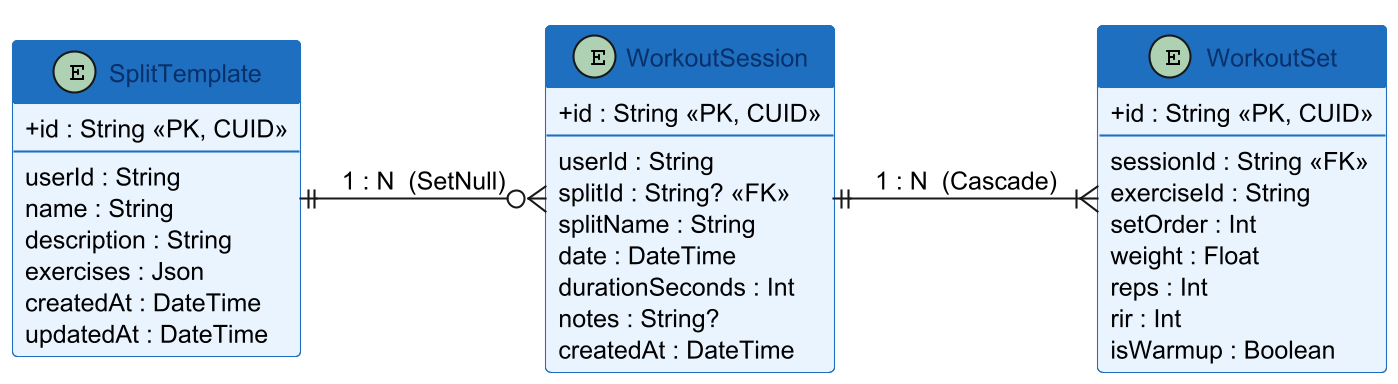
\includegraphics[width=\textwidth]{bazadedate.png}
  \caption{Diagrama entitate-rela\c tie a bazei de date}
  \label{fig:bazadedate}
\end{figure}

Cele trei modele formeaz\u a o ierarhie clar\u a:

\begin{itemize}
  \item Un utilizator (identificat prin \texttt{userId} Clerk) poate
        de\c tine orice num\u ar de \texttt{SplitTemplate}-uri \c si
        \texttt{WorkoutSession}-uri.
  \item O \texttt{WorkoutSession} poate fi asociat\u a cu cel mult
        un \texttt{SplitTemplate} (op\c tional).
  \item O \texttt{WorkoutSession} con\c tine unul sau mai multe
        \texttt{WorkoutSet}-uri.
\end{itemize}

Izolarea datelor \^ intre utilizatori este garantat\u a la nivelul
aplica\c tiei: toate interog\u arile Prisma includ filtrul
\texttt{where: \{ userId \}} extras din tokenul de autentificare
Clerk, astfel \^ inc\^ at un utilizator nu poate accesa datele
altui utilizator.

\section{API-ul REST}

Serverul Express expune un API REST cu dou\u a grupuri de endpoint-uri,
ambele protejate prin middleware-ul de autentificare Clerk.

\subsection{Endpoint-uri pentru rutine (\texttt{/api/splits})}

\begin{table}[htbp]
\centering
\caption{Endpoint-urile API pentru gestionarea rutinelor}
\label{tab:api-splits}
\begin{tabular}{|l|l|l|}
\hline
\textbf{Metod\u a} & \textbf{Rut\u a} & \textbf{Descriere} \\
\hline
GET    & \texttt{/api/splits}     & Returneaz\u a toate rutinele utilizatorului \\
POST   & \texttt{/api/splits}     & Creeaz\u a o rutin\u a nou\u a \\
PUT    & \texttt{/api/splits/:id} & Actualizeaz\u a o rutin\u a existent\u a \\
DELETE & \texttt{/api/splits/:id} & \c Sterge o rutin\u a \\
\hline
\end{tabular}
\end{table}

Endpoint-ul \texttt{POST /api/splits} valideaz\u a corpul cererii
cu schema Zod, verific\^ and c\u a rutina con\c tine un nume
nenul, o descriere op\c tional\u a \c si cel pu\c tin un exerci\c tiu
cu \texttt{exerciseId}, \texttt{targetSets} \c si
\texttt{targetRepRange} valide. Endpoint-urile
\texttt{PUT} \c si \texttt{DELETE} verific\u a suplimentar c\u a
resursa solicitat\u a apar\c tine utilizatorului curent,
return\^ and HTTP 404 \^ in caz contrar.

\subsection{Endpoint-uri pentru sesiuni (\texttt{/api/sessions})}

\begin{table}[htbp]
\centering
\caption{Endpoint-urile API pentru gestionarea sesiunilor}
\label{tab:api-sessions}
\begin{tabular}{|l|l|l|}
\hline
\textbf{Metod\u a} & \textbf{Rut\u a} & \textbf{Descriere} \\
\hline
GET  & \texttt{/api/sessions} & Returneaz\u a toate sesiunile utilizatorului \\
POST & \texttt{/api/sessions} & Salveaz\u a o sesiune nou\u a cu toate seturile \\
\hline
\end{tabular}
\end{table}

Endpoint-ul \texttt{POST /api/sessions} prime\c ste \^ intr-o
singur\u a cerere toate datele sesiunii: metadatele
(dat\u a, durat\u a, note, rutin\u a asociat\u a) \c si lista
complet\u a a seturilor efectuate. Crearea sesiunii \c si
a seturilor asociate se face \^ intr-o singur\u a tranzac\c tie
Prisma (\texttt{create} cu \texttt{sets: \{ create: [...] \}}),
garant\^ and atomicitatea opera\c tiei -- fie se salveaz\u a
totul, fie nimic.

Endpoint-ul \texttt{GET /api/sessions} returneaz\u a sesiunile
ordonate descendent dup\u a dat\u a, \^ impreun\u a cu seturile
asociate ordonate dup\u a \texttt{setOrder}.

Figura \ref{fig:secventa} ilustreaz\u a, sub forma unei diagrame de
secven\c t\u a, fluxul complet declan\c sat la salvarea unui antrenament:
de la trimiterea cererii de c\u atre client, p\^ an\u a la validarea
tokenului prin Clerk, validarea datelor cu Zod, scrierea \^ in baza de
date prin Prisma \c si returnarea r\u aspunsului.

\begin{figure}[htbp]
  \centering
  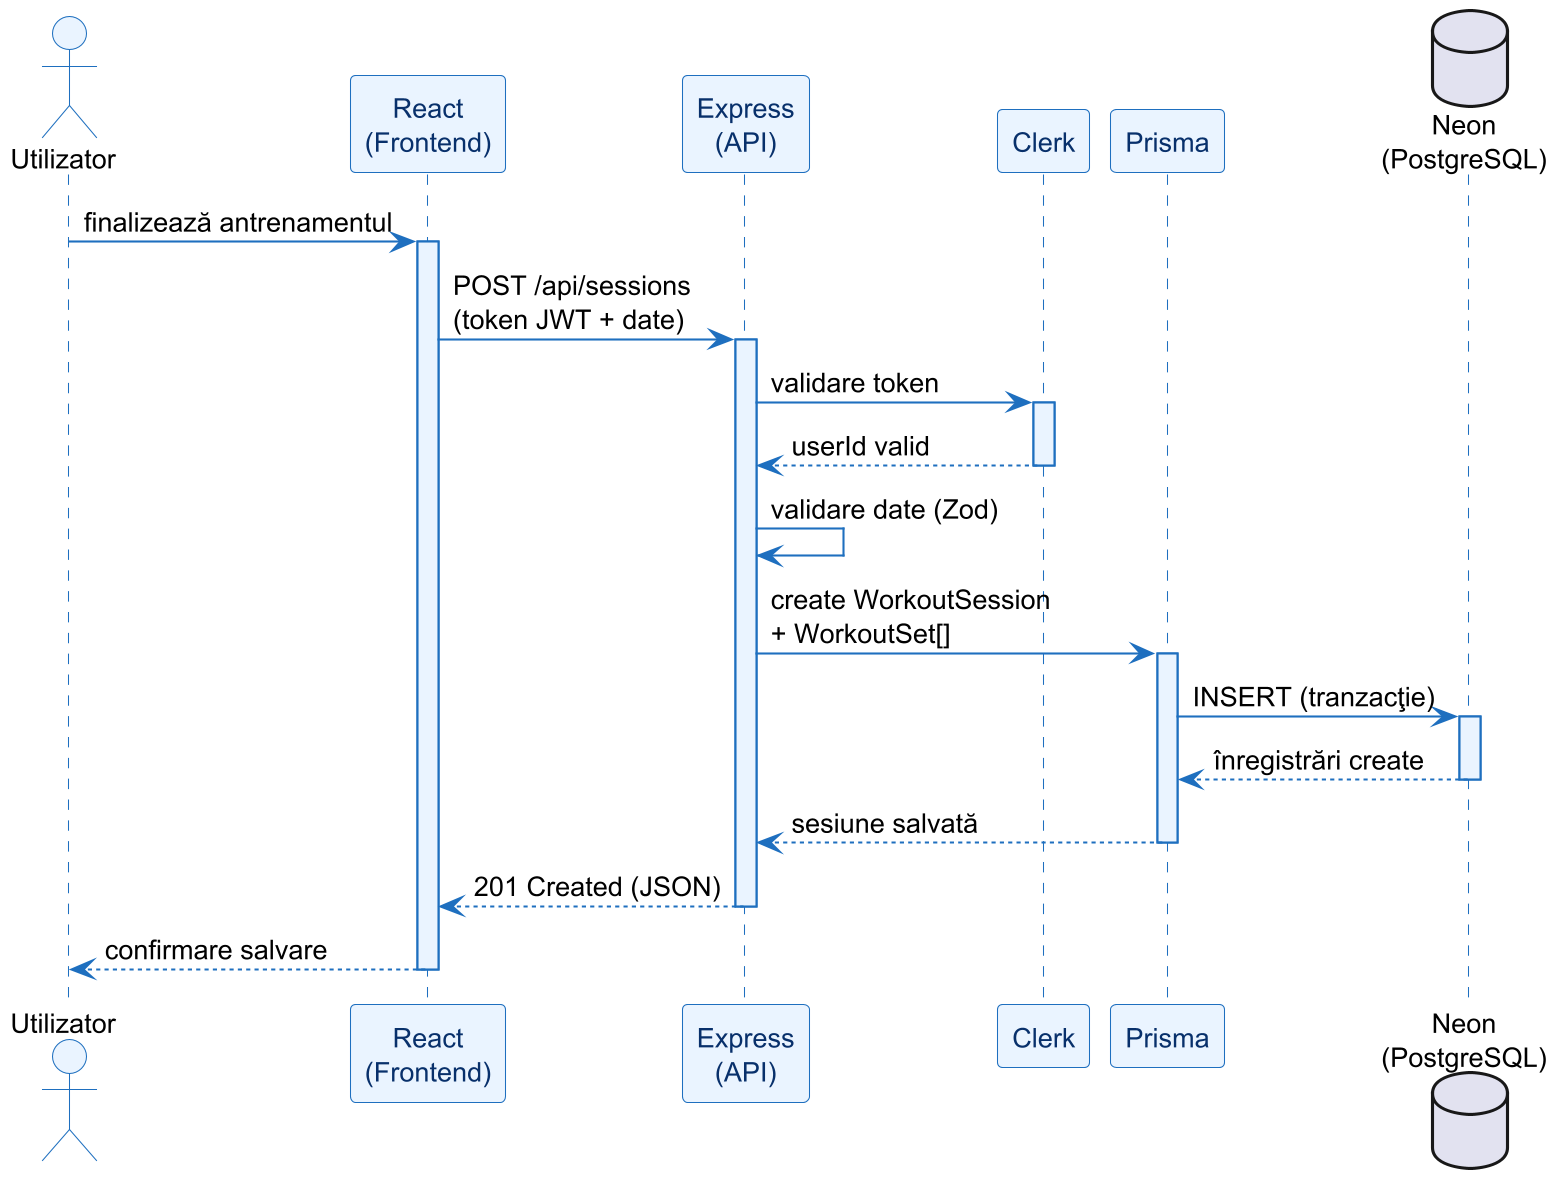
\includegraphics[width=\textwidth]{secventa.png}
  \caption{Diagrama de secven\c t\u a pentru salvarea unei sesiuni de antrenament}
  \label{fig:secventa}
\end{figure}

\section{Autentificarea \c si securitatea}

Autentificarea \^ in Gym-Connect este gestionat\u a integral
de serviciul \textbf{Clerk}, care furnizeaz\u a at\^ at
componentele UI de login/register, c\^ at \c si mecanismul
de validare a sesiunilor pe server.

\subsection{Fluxul de autentificare}

Fluxul de autentificare func\c tioneaz\u a \^ in urm\u atorii pa\c si:

\begin{enumerate}
  \item Utilizatorul se autentific\u a prin interfa\c ta Clerk
        (email + parol\u a sau OAuth).
  \item Clerk emite un \textbf{JWT} (\textit{JSON Web Token})
        semnat cu cheia privat\u a a aplica\c tiei.
  \item La fiecare cerere HTTP c\u atre server, clientul React
        include automat acest token \^ in header-ul
        \texttt{Authorization}.
  \item Pe server, middleware-ul \texttt{clerkMiddleware()}
        valideaz\u a tokenul \c si populeaz\u a obiectul cererii
        cu datele utilizatorului autentificat.
  \item Middleware-ul \texttt{requireAuth} extrage
        \texttt{userId} din cerere; dac\u a acesta lipse\c ste,
        returneaz\u a HTTP 401.
\end{enumerate}

\subsection{Middleware-ul de autentificare}

Middleware-ul \texttt{requireAuth} este aplicat global pe
toate rutele API \c si are urm\u atoarea logic\u a:

\begin{enumerate}
  \item Extrage \texttt{userId} din contextul Clerk al cererii
        curente folosind func\c tia \texttt{getAuth(req)}.
  \item Dac\u a \texttt{userId} este absent (utilizator
        neautentificat sau token expirat), returneaz\u a
        imediat r\u aspunsul \texttt{401 Unauthorized}
        cu mesajul \textit{,,Autentificare necesar\u a''}.
  \item Dac\u a autentificarea este valid\u a, adaug\u a
        \texttt{userId} pe obiectul cererii \c si transfer\u a
        controlul c\u atre handler-ul rutei.
\end{enumerate}

Prin aceast\u a abordare, nicio rut\u a API nu poate fi
accesat\u a f\u ar\u a un token valid, iar \texttt{userId}
este extras exclusiv din tokenul verificat de Clerk, nu
din parametrii cererii -- elimin\^ and posibilitatea
falsific\u arii identit\u a\c tii.

\subsection{Protec\c tia rutelor \^ in frontend}

\^ In frontend, rutele private sunt protejate prin componenta
\texttt{ProtectedRoute}, care utilizeaz\u a hook-ul
\texttt{useAuth()} al Clerk pentru a verifica starea de
autentificare. Dac\u a utilizatorul nu este autentificat,
este redirijat automat c\u atre pagina de autentificare.
\^ In caz contrar, componenta afi\c seaz\u a con\c tinutul
paginii solicitate.

\section{Diagrama cazurilor de utilizare}

Pentru a sintetiza interac\c tiunile posibile dintre utilizator \c si
aplica\c tie, figura \ref{fig:usecase} prezint\u a diagrama cazurilor
de utilizare (\textit{use-case}). Aceasta distinge \^ intre dou\u a
tipuri de actori: utilizatorul neautentificat, care poate doar s\u a
\^ i\c si creeze un cont sau s\u a se autentifice, \c si utilizatorul
autentificat, care are acces la \^ intreaga func\c tionalitate a
aplica\c tiei.

\begin{figure}[htbp]
  \centering
  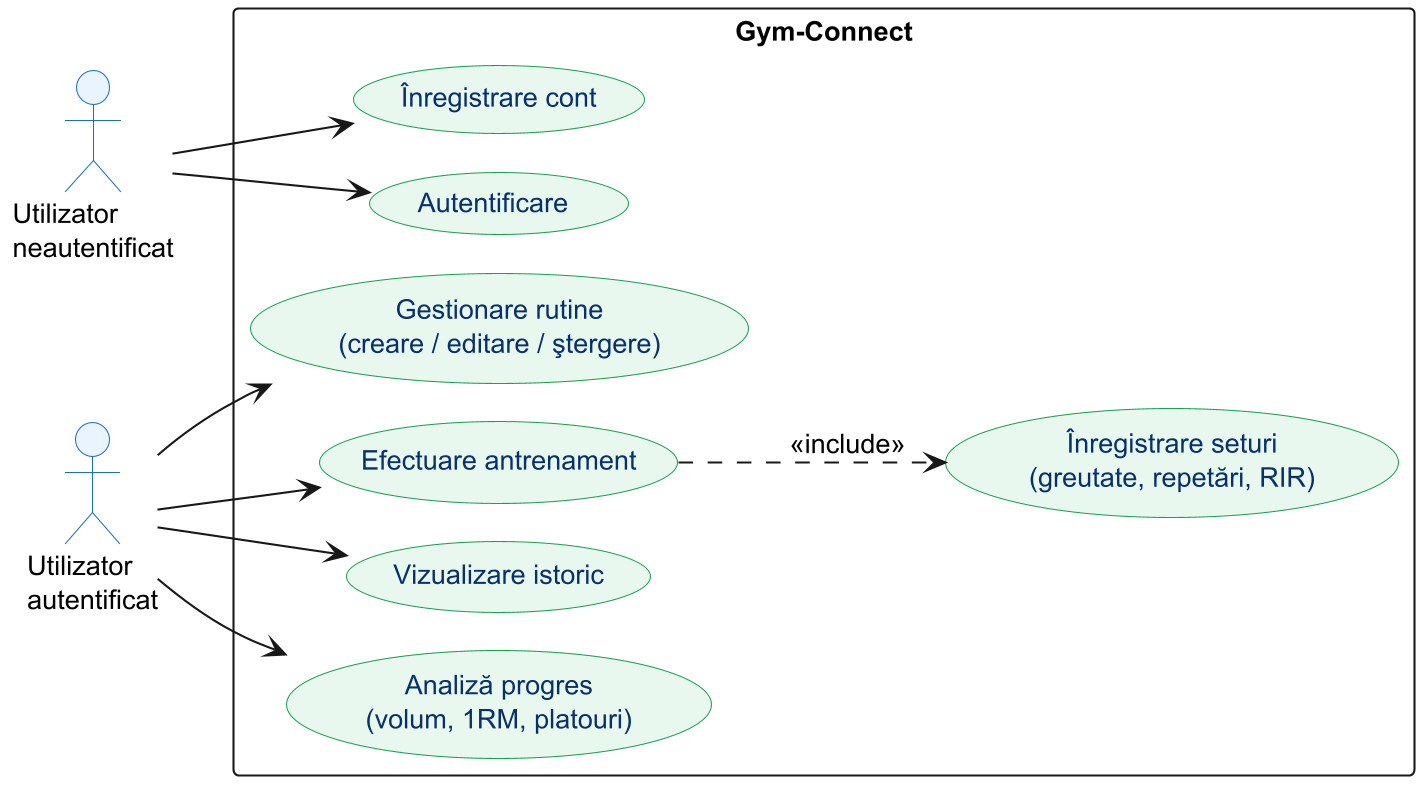
\includegraphics[width=\textwidth]{usecase.png}
  \caption{Diagrama cazurilor de utilizare a aplica\c tiei Gym-Connect}
  \label{fig:usecase}
\end{figure}

Dup\u a autentificare, utilizatorul poate gestiona rutine de
antrenament (creare, editare, \c stergere), poate efectua un
antrenament -- caz care include obligatoriu \^ inregistrarea
seturilor cu greutate, repeti\c tii \c si RIR -- poate vizualiza
istoricul sesiunilor anterioare \c si poate analiza progresul
prin intermediul modulului de analitic\u a.

